\section{Personnages}
Les personnages avec un ‘ \textbf{*} ’ sont des Jokers, ils possèdent un fiche de perso jouable. 

Par ordre d’apparition :

\newpage
\subsection{Aphra} \label{sec:aphra}
\begin{figure}[h!]
    \centering
    
\includegraphics[height=250pt]{_img/pnjs/aphra.png}
\end{figure}
\subsubsection{Background}
Chelli Lona Aphra, nommée d’après sa défunte mère Lona Aphra, surnommée Boop par son père, et appelée Aphra par le reste du monde, était une archéologue et contrebandière. Elle travailla notamment pour Dark Vador après la destruction de l’Étoile de la Mort. Jeune femme séduisante au tempérament bien trempé, brune avec des électrotatouages sur le bras droit, elle sait ce qu’elle veut, admire les gens de pouvoir, et ne fait confiance qu’à elle-même pour survivre. 

\subsubsection{Traits}

\begin{itemtable}[ c c c c c ]
    \textbf{Agi} & \textbf{Int} & \textbf{\^Ame} & \textbf{For} & \textbf{Vig} \\
    d8           & d12          & d4             & d6           & d6           
\end{itemtable}
\begin{itemtable}[ l X ]
    \textbf{Allure}      & 6 \\
    \textbf{Compétences} & Connaissance(Archéologie) d10, Réparation d10, Tir d8 \\
    \textbf{Atouts}      & Bidouilleur, Voleur, Acolyte(Wookie)
\end{itemtable}

\subsubsection{Défense}
\begin{itemtable}[ c c ]
    \textbf{Parade}     & \textbf{Résistance} \\
    6                   & 5 
\end{itemtable}

\newpage
\subsection{Reine de Ktath’Atn} \label{sec:ktath-atn-queen}
\begin{figure}[h!]
    \centering
    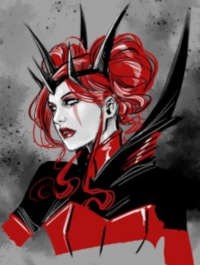
\includegraphics[height=250pt]{_img/pnjs/ktath-atn-queen.png}
\end{figure}
\subsubsection{Background}
Femme mystérieuse qui dirige la \textbf{Citadelle Hurlante} sur la planète Ktath’atn en l’an 0. Chaque année, elle organise une soirée durant laquelle elle reçoit de nombreux civils venus lui présenter des formes de vie organiques "intéressantes". Celui qui présente la forme de vie la plus intéressante se voit alors accorder un veux par la reine.

\subsubsection{Traits}

Sa \textbf{Vig}ueur dépend depuis combient de temps elle s’est nourrir. 

\begin{itemtable}[ c c c c c ]
    \textbf{Agi} & \textbf{Int} & \textbf{\^Ame} & \textbf{For} & \textbf{Vig} \\
    d10           & d10         & d4             & d4           & d8           
\end{itemtable}
\begin{itemtable}[ l X ]
    \textbf{Allure}      & 6 \\
    \textbf{Compétences} & Intimidation d8, Persuasion d8, Réseaux d10, Combat d8 \\
    \textbf{Atouts}      & Commandement
\end{itemtable}

\subsubsection{Défense}
\begin{itemtable}[ c c ]
    \textbf{Parade}     & \textbf{Résistance} \\
    6                   & 6 
\end{itemtable}

\newpage

\subsection{Bombinax} \label{sec:bombinax}
\begin{figure}[h!]
    \centering
    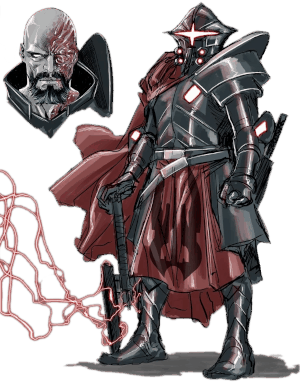
\includegraphics[height=250pt]{_img/pnjs/bombinax.png}
\end{figure}
\newpage

\subsection{Varroa} \label{sec:varroa}
\newpage
\subsection{Vespinax} \label{sec:vespinax}
